\documentclass[11pt]{article}

\usepackage{amsmath,amssymb}
\usepackage{geometry}
\geometry{margin=20mm}
\usepackage{graphicx}
\usepackage{subcaption}
\usepackage[T1]{fontenc}
\usepackage{babel}


\title{Investigating the applications and limits of single particle light scattering using limited detection schemes}

\author{Maciver, Daniel}
	
\begin{document}
	
\maketitle

\section*{Abstract}
Obtaining Static Light Scattering profiles from optically trapped entities poses considerable engineering challenge due to space constraints in a typical Optical Trap setup. We propose here a three-angle light scattering technique that can not only help characterize the structure but also be useful in understanding the dynamics of microscopic objects that are trapped optically. In this work, we demonstrate the use of such a measurement scheme in determining the optimal angles for light scattering measurements and probing the orientational dynamics of a microsphere dimer. 

\section*{Introduction}
Optical trapping has been a vital tool in the study of single molecule properties, the ability to deliver a stable and precise force vector has proved invaluable for studying biological groups in particular \cite{2}. Recent years there has been a growing interest in the study of colloid aggregation and growth; where the optical binding effect resulted in rapid aggregation of nanoparticles around the trapping focus. Raman scattering techniques can be used to elucidate particle characteristics and have been applied to optical trapping methods to determine compositional information of the trapped entity \cite{4,7}. However, the particle's dynamics in the trap can not be elucidated based purely on the spectral data. For simple near spherical particles the motion can be largely attributed to Brownian motion which can be readily measured using a quadrant photo detector. It is not unusual however, that two microspheres to become attached to one another; in the presence of a focused Gaussian beam the microsphere dimer will reorient itself to align along the propagation axis of the beam. If the dimer is symmetrical then this reorientation motion is instantaneous, in the case of an asymmetrical dimer the alignment rapidly fluctuates about the propagation axis before eventually achieving an equilibrated orientation. Developing a method to model a dimer's motion within an optical trap based on information gathered in situ will prove useful for understanding the dynamics of more complexly shaped particle's that cannot be directly imaged.

This has already been achieved with single microsphere using dynamic light scattering measurements of the trapping beam; where Bar-Ziv et al utilised dynamic light scattering to characterise the trap's stiffness and anisotropy based on the Brownian motion of a trapped silica microsphere \cite{1}. They note that their method assumes that the silica scatters isotropically which allows them to place a single detection fibre at $75^\circ$ from the propagation axis. In the case where the trapped object scatters anisotropically - such as for an asymmetrical dimer - it is necessary to utilise multiple detection fibres to build a better picture of the trapped object's orientation based on the produced light scattering. However, for inverted microscope optical traps there is a significant engineering challenge of placing enough detection fibres at the correct angles within a close enough distance to the trapping focus to collect a clear signal. This means that any fibre based detection will have to rely on maximising the information provided by the light scattering signals collected at a limited number of detection fibres. Excluding the engineering challenge involved with ensuring proper coupling between the probe laser and the detection fibres, the primary concern is how much useful information can be extracted from the trapped particle. 

We are currently developing an experimental set up that will allow us to light scattering 

\section*{Theory}

Consider a dimer with unequal sphere diameters $a_1, a_2$ in an optical trap positioned in some orientation $\hat{s}$. Due to the Brownian motion from the surrounding fluid the dimer's orientation changes with time. Assuming we cannot accurately determine the dimer's orientation from imaging alone we instead rely on it's light scattering. We collect the near field intensity, via optical fibres,from a probe laser at 3 predetermined angles $\theta_1, \theta_2, \theta_3$. To determine the particle's orientation we compare the produced light scattering signal to a collection of reference orientations that are evenly spaced around the orientation space.   
\begin{figure}
	\begin{subfigure}{0.45\textwidth}
			\begin{tabular}{rrrr}
				\hline\hline
				orientation & $\hat{n}_x$ &  $\hat{n}_y$ &  $\hat{n}_z$ \\
				\hline
				$1$ & $ 0.29588$ &  $ 0.29588$ & $ 0.90825$ \\
				$2$ & $ 0.90825$ &  $ 0.29588$ & $ 0.29588$ \\
				$3$ & $ 0.29588$ &  $ 0.90825$ & $ 0.29588$ \\
				$4$ & $ 0.29588$ &  $ 0.29588$ & $-0.90825$ \\
				$5$ & $ 0.90825$ &  $ 0.29588$ & $-0.29588$ \\
				$6$ & $ 0.29588$ &  $ 0.90825$ & $-0.29588$ \\
				$7$ & $ 0.29588$ &  $-0.29588$ & $ 0.90825$ \\
				$8$ & $ 0.90825$ &  $-0.29588$ & $ 0.29588$ \\
				$9$ & $ 0.29588$ &  $-0.90825$ & $ 0.29588$ \\
				$10$ & $ 0.29588$ &  $-0.29588$ & $-0.90825$ \\
				$11$ & $ 0.90825$ &  $-0.29588$ & $-0.29588$ \\
				$12$ & $ 0.29588$ &  $-0.90825$ & $-0.29588$ \\
				$13$ & $-0.29588$ &  $ 0.29588$ & $ 0.90825$ \\
				$14$ & $-0.90825$ &  $ 0.29588$ & $ 0.29588$ \\
				$15$ & $-0.29588$ &  $ 0.90825$ & $ 0.29588$ \\
				$16$ & $-0.29588$ &  $ 0.29588$ & $-0.90825$ \\
				$17$ & $-0.90825$ &  $ 0.29588$ & $-0.29588$ \\
				$18$ & $-0.29588$ &  $ 0.90825$ & $-0.29588$ \\
				$19$ & $-0.29588$ &  $-0.29588$ & $ 0.90825$ \\
				$20$ & $-0.90825$ &  $-0.29588$ & $ 0.29588$ \\
				$21$ & $-0.29588$ &  $-0.90825$ & $ 0.29588$ \\
				$22$ & $-0.29588$ &  $-0.29588$ & $-0.90825$ \\
				$23$ & $-0.90825$ &  $-0.29588$ & $-0.29588$ \\
				$24$ & $-0.29588$ &  $-0.90825$ & $-0.29588$ \\
				\hline\hline
			\end{tabular}
	\end{subfigure}
	\begin{subfigure}{0.45\textwidth}
		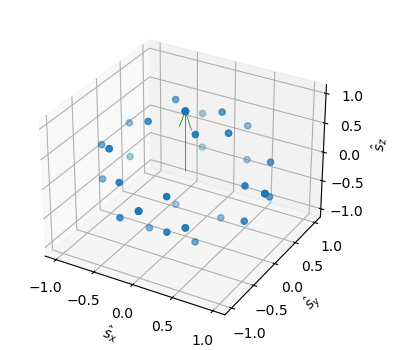
\includegraphics[width=1.35\textwidth]{junk_00000.png}
	\end{subfigure}
\caption{Reference orientations plotted in the physical space. Green arrow points in the direction of the dimers orientation.}
\end{figure}

We use the a Fortran package specialised for calculating non spherical t-matrices (MSTM) \cite{6} to determine the light scattering intensity of our dimer in each reference orientation. We assume that the for each detection fibre the intensities can be distributed on a Gaussian curve centred at $y_k$, the normalised intensity at detection fibre k. Based on the light scattering from the dimer we can assign a probability that the produced light scattering pattern produced belongs to the reference orientation $\hat{n}$

\begin{align}
	p(y(\hat{s})\parallel\hat{n}) = \Pi^3_{k=1} 
	(2\pi\sigma_k^2)^{-1/2} e^{-(y(\hat{n})_k-y(\hat{s})_k)^2/2\sigma_k^2}
\end{align}

Where $\sigma_k$ is the average error in our signal collection; we assumed that in a best case scenario for our set up there will be roughly a $17\%$ error in the signal we collected. This was implemented by adjusting the values of $y(\hat{s}_k)$. 
\begin{eqnarray*}
	\sigma_k = 0.17\bar{y}(\hat{n}_k) \\
	\Rightarrow y(\hat{s}_k) = y(\hat{s})_k \pm n\sigma_k \\ 
	n \in \mathbb{R}, n\in[0,1]
\end{eqnarray*}
	
We can view this result as a conditional probability, if the orientation is determined ($\hat{n}$) then what is the probability that expected scattering signal matches our dimer's scattering signal. We instead want to know the inverse conditional, that with a given signal y the dimer was in orientation $\hat{n}$. We can calculate this using Bayes' theory:

\begin{align}
	p(\hat{n}\parallel y(\hat{s})) = \frac{p(y(\hat{s})\parallel\hat{n})p(\hat{n})}{p(y)}
\end{align}

Where $p(\hat{n})$ and $p(y)$ are our estimations of the priori distributions of particle orientations and scattering signals respectively. The former can be estimated by some Boltzmann distribution based on the radial distance between neighbouring reference orientations. This essentially is biasing our estimate by tying it to its proximity in the orientation space. The latter priori can be taken as the integral of  $p(y(\hat{s})\parallel \hat{n})$ and $p(\hat{n})$ across all possible reference orientations. In order to evaluate if our model is accurate we need first test it using an idealised simulation of the target dimer. 

\subsection*{Testing the model}
We use the Brownian OT package by Jerome Fung \cite{5} to simulate how our target dimer moves while subject to an optical trap. At each time step we determine the dimer's orientation and use MSTM to calculate its scattering pattern. We then use the above method to estimate the dimer orientation based on its scattering pattern. The priori estimate of the particle's orientation can be defined as a Boltzmann's distribution based on the radial distance between our previous estimate and each reference orientation. 
\begin{align}
	r_j(t, \hat{n}) = \hat{n}_{t} \cdot \hat{n}_{t-\Delta t} \\
	p(\hat{n}) = \frac{e^{r_j(t,\hat{n})}}
	{\Sigma_{i=1}^{24}e^{r_i(t, \hat{n})}}
\end{align}

Since we are testing with a simulation we already know the exact orientation of the dimer, we want to know if our model can correctly predict the closest reference orientation. We take the dot product between our estimated $\hat{n}$ and the correct $\hat{n}$ and calculate the angle between the two. Performing a summation over the full simulation data we should see that the model has a total  

$$  K_l(B \parallel D) = - \sum_{n=1}^{no. steps} B_n \ln(\frac{D_n}{B_n})$$


Where $B_n$ is the Bayesian estimate and $D_n$ is the dot product result; the closer our estimate is to the dot product result the more accurate the model, and the divergence will approach 0. We can therefore evaluate the overall accuracy of our estimate based on the divergence - which is determined primarily by the detection angles. 

\subparagraph*{Measurement of divergence parameter space}
The efficacy of our estimation is a function of our detection angles, testing every possible configuration manually is time consuming, therefore we utilised Ultra nest to apply a Monte Carlo simulation to our model. 

Ultra-nest is a sophisticated python package for fitting models with complex parameter interactions \cite{3}. Basic fitting methods (i.e. sum of least squares) are intended for finding the parameter choice with the best overall fit to the data. While this works well for functions with few fitting parameters and where the parameters are already constrained to predefined values; the computation time required for more functions where the parameters are less constrained and/or have no direct connection to the final returned result. 

In cases like this its best to implement Monte Carlo techniques to intelligently sample across the entire parameter space. Ultra-nest implements a variation of this called nested-sampling, where the likelihood contour is used to update a group of live points chosen from the prior estimation.

\section*{Results}
\subparagraph*{Asymmetric dimer dynamics}
The Brownian OT software was used to simulate the motion of a trapped dimer ($a_1=1\mu m, a_2=0.5\mu m$) over the first 10 seconds of entering the optical trap. The initial orientation was assumed as strictly vertical (in line with the beam propagation direction). The dimer's position orientation was recorded every $10 \mu s$ for using as a test dataset for our model. 

\begin{figure}[h]
	\centering
	\begin{subfigure}{0.45\textwidth}
		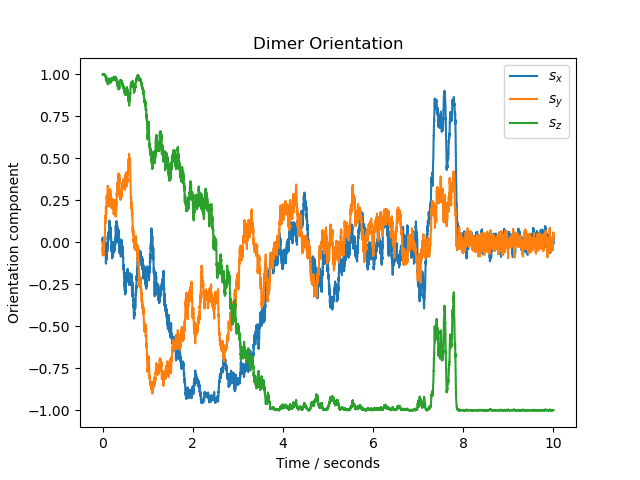
\includegraphics[width =\textwidth]{traj.png}
	\end{subfigure}
	\begin{subfigure}{0.45\textwidth}
		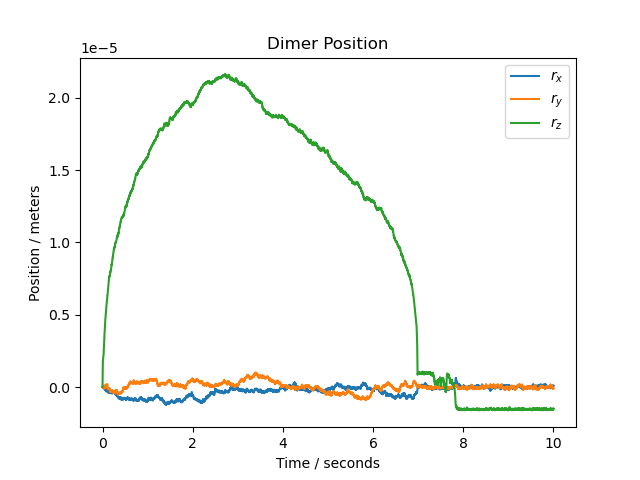
\includegraphics[width=\textwidth]{pos.png}
	\end{subfigure}
	\caption{Simulation results of: a) the dimers orientation vector with time, b) the dimer's [x,y,z] position with time.}
\end{figure}

As can be seen from Figure 2, the dimer undergoes a full $180^{\circ}$ rotation upon entering the trap. Typically horizontal alignment of a dimer is unstable and will result in the particle rotating to align along its vertical axis. It is interesting to note that the dimer is furthest from the trap centre as it goes into a horizontal orientation before drawing closer again as it inverts completely. Further simulations of differently sized dimers showed similar results, but only when $a_1 \geq 2a_2$. Dimers with more symmetrical size ratios immediately aligned into a fixed vertical position. 
In Vigilante's work with dimers \cite{5} simulations of trapped symmetrical dimers was investigated; their findings showed that the optical torque on the dimer goes to zero while aligned vertically and is at its maximum in a horizontal alignment. Therefore, the inversion of an asymmetric dimer suggests that if the size difference is significant the optical torque goes is minimal for a dimer in both horizontal and vertical orientations. 

\subparagraph*{Predictive efficacy of model}
The data from Figure 2a was used to test the efficacy of our predictive model. By recording how much our estimate diverges from the true orientation we get a rough score of how well our model can predict the dimer's orientation.

\begin{figure}[h]
	\centering
	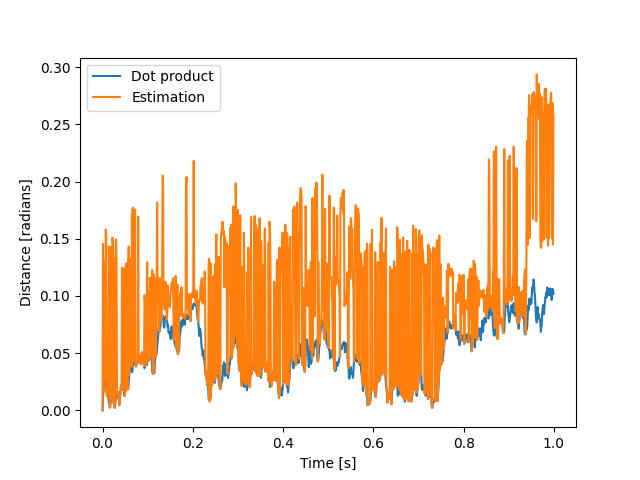
\includegraphics[width=0.5\textwidth]{Divergance.png}
	\caption{Divergence between our model estimate and best estimate calculated via taking the dot product}
\end{figure}

Spikes in the divergence plot indicate that the model is deviating  from the desired prediction. From Figure 3 we can see our model has short bursts of being highly accurate in its prediction before suddenly shooting off. This can be in part be due to the fact that our $y(\hat{s}_k)$ values are not set but fluctuate due to the signal error. Reduction of the signal error results in a higher accuracy in the models predictive efficacy to an extent; in truth the most significant factor in the prediction is our priori estimate of the dimer orientation $p(\hat{n})$. Since our choice of reference orientations have mirror copies in the physical space the conditional probabilities $p(y_k\parallel\hat{n})$ can be very close to each other. The addition of $p(\hat{n})$ means results in a significant improvement in the prediction by restraining our result to orientations close together in the physical space. 

\section*{Conclusion}
We have developed a model for interpreting the dynamics of a trapped particle based purely on the light scattering pattern. The 

\bibliography{bib}
\bibliographystyle{ieeetran}
\end{document}
